%%%%%%%%%%%%%%%%%%%%%%%%%%%%%%%%%%%%%%%%%%%%%%%%%%%%%%%%%%%%%%%%%%%%%%%%%%%%%%%%
%%%%%%%%%%%%%%%%%%   Vorlage für eine Abschlussarbeit   %%%%%%%%%%%%%%%%%%%%%%%%
%%%%%%%%%%%%%%%%%%%%%%%%%%%%%%%%%%%%%%%%%%%%%%%%%%%%%%%%%%%%%%%%%%%%%%%%%%%%%%%%

% Erstellt von Maximilian Nöthe, <maximilian.noethe@tu-dortmund.de>
% ausgelegt für lualatex und Biblatex mit biber

% Kompilieren mit
% lualatex dateiname.tex
% biber dateiname.bcf
% lualatex dateiname.tex
% lualatex dateiname.tex
% oder einfach mit:
% make

\documentclass[
  12pt,
  tucolor,
  BCOR=12mm,     % 12mm binding corrections, adjust to fit your binding
  parskip=half,  % new paragraphs start with half line vertical space
  open=any,      % chapters start on both odd and even pages
  cleardoublepage=plain,  % no header/footer on blank pages
]{tudothesis}

\usepackage{setspace}
\usepackage[a4paper, left=2.5cm, right=2.5cm, top=3.5cm, bottom=3.5cm]{geometry}


% Warning, if another latex run is needed
\usepackage[aux]{rerunfilecheck}

% just list chapters and sections in the toc, not subsections or smaller
\setcounter{tocdepth}{1}

%------------------------------------------------------------------------------
%------------------------------ Sprache und Schrift: --------------------------
%------------------------------------------------------------------------------
\usepackage{mathptmx}
\usepackage{fontspec}
\defaultfontfeatures{Ligatures=TeX}  % -- becomes en-dash etc.

% german language
\usepackage{polyglossia}
\setdefaultlanguage{german}

% for english abstract and english titles in the toc
\setotherlanguages{english}

% intelligent quotation marks, language and nesting sensitive
\usepackage[autostyle]{csquotes}

% microtypographical features, makes the text look nicer on the small scale
\usepackage{microtype}

%------------------------------------------------------------------------------
%------------------------ Für die Matheumgebung--------------------------------
%------------------------------------------------------------------------------

\usepackage{amsmath}
\usepackage{amssymb}
\usepackage{mathtools}

% Enable Unicode-Math and follow the ISO-Standards for typesetting math
\usepackage[
  math-style=ISO,
  bold-style=ISO,
  sans-style=italic,
  nabla=upright,
  partial=upright,
]{unicode-math}
\setmathfont{Latin Modern Math}

% nice, small fracs for the text with \sfrac{}{}
\usepackage{xfrac}


%------------------------------------------------------------------------------
%---------------------------- Numbers and Units -------------------------------
%------------------------------------------------------------------------------

\usepackage[
  locale=DE,
  separate-uncertainty=true,
  per-mode=symbol-or-fraction,
  binary-units=true
]{siunitx}
\sisetup{math-micro=\text{µ},text-micro=µ}

%------------------------------------------------------------------------------
%-------------------------------- tables  -------------------------------------
%------------------------------------------------------------------------------

\usepackage{booktabs}       % stellt \toprule, \midrule, \bottomrule

%------------------------------------------------------------------------------
%-------------------------------- graphics -------------------------------------
%------------------------------------------------------------------------------

\usepackage{graphicx}
\usepackage{grffile}

% allow figures to be placed in the running text by default:
\usepackage{scrhack}
\usepackage{float}
\floatplacement{figure}{htbp}
\floatplacement{table}{htbp}

% keep figures and tables in the section
\usepackage[section, below]{placeins}


%------------------------------------------------------------------------------
%---------------------- customize list environments ---------------------------
%------------------------------------------------------------------------------

\usepackage{enumitem}

%------------------------------------------------------------------------------
%------------------------------ Bibliographie ---------------------------------
%------------------------------------------------------------------------------

\usepackage[
  backend=biber,   % use modern biber backend
  autolang=hyphen, % load hyphenation rules for if language of bibentry is not
                   % german, has to be loaded with \setotherlanguages
                   % in the references.bib use langid={en} for english sources
]{biblatex}
\addbibresource{references.bib}  % die Bibliographie einbinden
\DefineBibliographyStrings{german}{andothers = {{et\,al\adddot}}}

%------------------------------------------------------------------------------
%------------------------------ Sonstiges: ------------------------------------
%------------------------------------------------------------------------------

\usepackage[pdfusetitle,unicode,linkbordercolor=tugreen]{hyperref}

\AtBeginDocument{%
\newcaptionname{ngerman}{\figureautorefname}{Abbildung}
\newcaptionname{ngerman}{\tableautorefname}{Tabelle}
\newcaptionname{ngerman}{\sectionautorefname}{Kapitel}
\newcaptionname{ngerman}{\chapterautorefname}{Kapitel}%
}

\usepackage{bookmark}
\usepackage[shortcuts]{extdash}
\usepackage{verbatim}

%------------------------------------------------------------------------------
%-------------------------    Angaben zur Arbeit   ----------------------------
%------------------------------------------------------------------------------

\author{Lars Möllerherm}
\title{Fake News Detektion}
\division{Fakultät Physik}
\submissiondate{31. August 2019}
\firstcorrector{Dr.~Olaf~Nackenhorst}
\secondcorrector{Dr.~Johannes~Erdmann}
\eventname{Maschinelles Lernen für Physiker*innen}

% tu logo on top of the titlepage
\titlehead{\includegraphics[height=1.5cm]{logos/tu-logo.pdf}}

\begin{document}
\onehalfspacing
\frontmatter
\maketitle

% Gutachterseite
\makecorrectorpage
\tableofcontents
\mainmatter
% Hier beginnt der Inhalt mit Seite 1 in arabischen Ziffern
\chapter{Motivation}
\label{sec:motivation}

Als Fake News werden Falschmeldungen bezeichnet, die mit manipulativer Absicht viral verbreitet werden. In dem 
"Whitepaper"\cite{facebook}, was Facebook am 27.04.2017 veröffentlichte, werden vier verschiedene Motive und  
Methoden von Falschnachrichten beschrieben. 
Zum einen die Verbreitung mit der Absicht, politische Stimmungen 
zu steuern, zum anderen mithilfe von Fehlinformationen bestimmt Gefühle zu erzeugen oder Aufmerksamkeit zu erzielen. 
Ein weitere Methode kann das Manipulieren von politischen Diskussionen mithilfe von koordinierten Aktivitäten sein und 
zu letzt die bloße Desinformation.

Die Motive und Methoden werden immer komplexer und aufgrund der hohen Lukrativität\cite{Cynk} wird es immer schwieriger 
ohne große Eigenrecherche zu erkennen, ob die Nachricht eine Falschmeldung darstellt.
Da eine Verbreitung in sozialen Netzwerken deutlich einfacher ist und diese Plattformen zunehmend als
Informationsquelle genutzt werden\cite{nachrichtenquelle}, wächst die Gefahr, die von Fake News ausgeht.
Durch die unaufhaltsame und selbstständige Verbreitung der Nachrichten in den Netzwerken, sind Falschnachrichten schwer 
zu revidieren und es sollte von Interesse sein den Wahrheitsgehalt schnell überprüfen zu können, um diese
zu verhindern.

Eine Überprüfung des Inhalts würde zu viel Zeit in Anspruch nehmen. Eine schnellere Möglichkeit wäre eine Analyse 
des Textes mithilfe von Natural Language Processing und einer anschließenden Klassifizierung mit Neuronalen Netzen.
Dabei werden sowohl Kontext als auch Schreibstil des Textes analysiert und dann anhand dieser Information eine 
Likelihood bestimmt, zu der ein Text "Fake" oder "Real" ist.
Diese Methode kann eine Überprüfung des Inhalts nicht ersetzen, 
jedoch könnte es bei einer ausreichenden Genauigkeit zu einem vorläufigen Sperren der Nachricht führen, was die 
unaufhaltsame Verbreitung verhindern würde.
Eine schon vorhandene Möglichkeit Fake News zu detektieren ist der "B.S. Detector" von Daniel Sieradski\cite{BS}.
Diese Browser Erweiterung überprüft alle in dem Artikel verlinkten Webseiten auf verdächtige Quellen, indem es die 
Domains mit einer manuell gepflegten Liste von unzuverlässigen Quellen vergleicht. 
Nachteile sind, dass verdächtige Quellen nicht unbedingt bedeuten, dass es sich um 
Falschnachrichten handelt und durch Vermeiden fragwürdiger Quellen kann die Detektion verhindert werden.


\chapter{Struktur und Verarbeitung des Datensatzes}
\label{sec:struct}

Der Datensatz besteht zu $44\,\%$ aus Nachrichten die vom B.S. Detektor detektiert wurden und zu $56\,\%$ aus gesammelten 
Nachrichten von vertrauenswürdigen Nachrichtendiensten, wie die Washington Post oder die New York Times. Die Nachrichten 
sind hauptsächlich auf Englisch und die Falschnachrichten sind vom 25. Oktober 2016 bis 25. November 2016 gesammelt worden. Für den Zeitraum 
der Real News ist Oktober bis November 2016 angegeben. 
Der Fake News Datensatz ist auf Kaggle.com zu finden\cite{fake_data} und die Real News werden in einem Kernel hinzugefügt\cite{real_data}.
Nach dem Aussortieren der nicht englischsprachigen Texte mithilfe der \textsc{langdetect}-Bibliothek\cite{langdetect}, welche die
Language Detection Bibliothek von Google\cite{google_langdetect} nutzt, hat der gesamte Datensatz eine Größe von 
$\num{27903}$ Nachrichten.

Aufgrund des gegebenen Datensatzes kann die Fragestellung dieser Arbeit nur eingeschränkt formuliert werden.
Mithilfe dieses Datensatzes kann keine allgemeine Fake News Erkennung trainiert werden, da hier nicht der Inhalt 
ausschlaggeben für die Klassifizierung der Trainingsdaten ist, sondern der B.S. Detektor und somit die Quellen des 
Artikels. 
Zudem gibt es in dem Real News Datensatz nur $10$ verschiedene Herausgeber.
Daher hat der Datensatz eine große Verzerrung und es kann nur darauf trainiert werden, ob Texte vom B.S. Detektor 
als fragwürdig klassifiziert werden würden oder ob sie von einem der $10$ als glaubwürdig erachteten Herausgebern stammt.
Zudem sind die Thematiken der Texte auf den Zeitraum Oktober bis November 2016 beschränkt.

Zunächst wird der Datensatz mithilfe der \textsc{nltk}-Bibliothek\cite{nltk} durch Lemmatisierung verarbeitet, um 
alle Wörter auf ihre Stammform zurückzuführen (siehe \autoref{sec:NLP}). 
Anschließend werden die Worthäufigkeiten in jedem Text mithilfe der \textsc{scikit-learn}-Bibliothek\cite{scikit-learn} 
gezählt. 
Somit ergibt sich das Bag-of-words Modell als Repräsentation des Textes.
Auf eine Aussortieren der Stoppwörter wird verzichtet, da diese zwar nicht relevant für den Inhalt der Nachricht sind,
jedoch Teil des Schreibstils sind und somit relevant für eine Trennung sein können.
Um zu generalisieren werden nur die $500$ im Trainingsdatensatz am häufigsten Verwendeten Wörter genutzt. 
Somit werden Wörter die nur in einzelnen Texten verwendet werden ignoriert und ein Übertraining ist schwieriger.

\begin{comment}
    \begin{figure}[t!]
    \centering
    \begin{subfigure}[t]{0.45\textwidth}
        \centering
        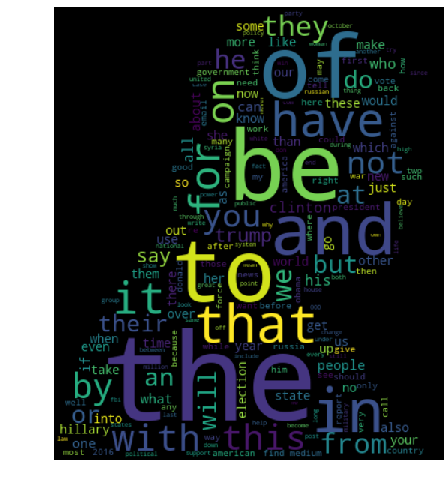
\includegraphics[width=\textwidth]{pictures/fake_wordcloud.pdf}
        \caption{Fake News}
    \end{subfigure}
    \begin{subfigure}[t]{0.54\textwidth}
        \centering
        \raisebox{1.5cm}[0pt]{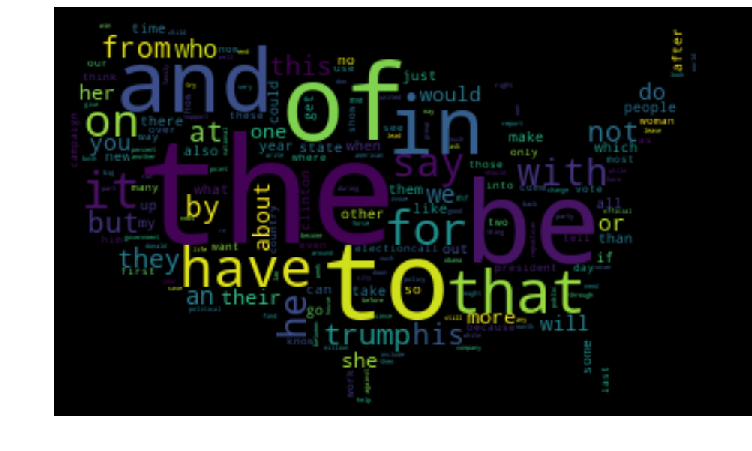
\includegraphics[width=\textwidth]{pictures/real_wordcloud.pdf}}
        \caption{Real News}
    \end{subfigure}
    \caption{Mit \textsc{wordcloud} \cite{wordcloud} erstellte Darstellung der Worthäufigkeiten für Real und Fake News.}
    \label{fig:wordcloud}
    \end{figure}
\end{comment}


\chapter{Lösungsansatz}
\label{sec:ansatz}

\begin{figure}
    \centering
    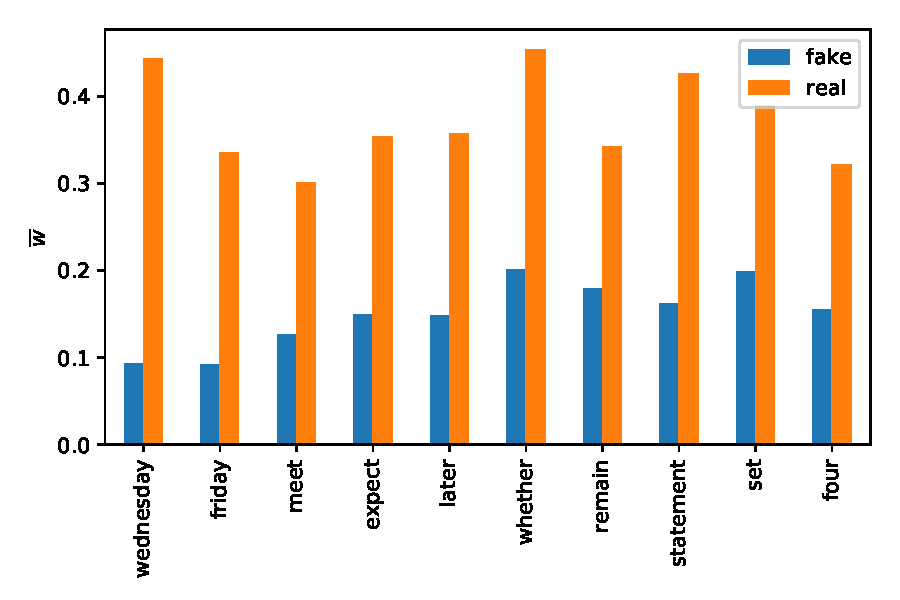
\includegraphics[width=0.8\textwidth]{pictures/data_visualisation.pdf}
    \caption{Darstellung der relativen Worthäufigkeit der $10$ Wörter, mit maximaler Differenz der Mittelwerte.
            Eine Unterschied ist klar zu erkennen, wobei ein Teil dadurch erklärt ist, dass die Texte der Real 
            News im Mittel $\approx 1590$ Zeichen länger sind.}
    \label{fig:word_plot}
\end{figure}

Um zu veranschaulichen, ob ein Unterschied der Worthäufigkeiten im Fake- und Real-News Datensatz besteht, werden in \autoref{fig:word_plot}
die $10$ Wörter der $500$ häufigsten Worten dargestellt, die am besten zur Trennung geeignet sind. 
Als Kriterium wird 
\begin{equation}
    \frac{(\overline{w_{real}}-\overline{w_{fake}})^2}{s_{real}^2+s_{fake}^2}
\end{equation}
verwendet, welches von der eindimensionalen linearen Fisher Diskriminanzanalyse inspiriert ist. 
Dabei ist $\overline{w_k}$ das arithmetische Mittel und $s_{k}^{2}=\frac{1}{N_k}\sum_{i=1}^{N_{k}}\left(w_{k i}-\overline{w}_{k}\right)^{2}$ 
die Stichproben Varianz.
Wörter mit großen Distanzen zwischen den Mittelwerten relativ zu der Streuung können gut zur Trennung genutzt werden, was 
jedoch nicht bedeutet, dass auch das Neuronale Netz diesen Wörtern großes Gewicht zuschreibt.
In \autoref{fig:word_plot} ist zu erkennen, dass Real und Fake News durchaus anhand der Worthäufigkeit zu unterscheiden sind. 
Da die Wörter in \autoref{fig:word_plot} nicht themenspezifischen sind, deutet es daraufhin, dass eine unterschiedliche 
Ausdrucksweise ausschlaggeben ist. 
Zum Beispiel scheinen Wochentage in den Real News häufiger verwendet zu werden. 
Das kann zum Teil daran liegen, dass bei Fakten ein genauer Zeitpunkt erwähnt werden kann und bei Falschnachrichten, die 
nur auf eine emotionale Reaktion zielen, ist der genaue Zeitpunkt des Ereignisses nicht existent und auch nicht relevant.
Zu beachten ist, dass Real News im Mittel $\num{1590}$ Zeichen länger sind als Fake News und somit Real News durchschnittlich
eine höhere relative Häufigkeit besitzen.
Dies ist jedoch auch ein Attribut, welches aus dem BoW Modell generiert und genutzt werden kann.
Des Weiteren scheinen Stoppwörter, wie "whether", relevant zu sein, weshalb sie mit in die Analyse genommen werden.

Die $500$ Wörter, die wie in \autoref{sec:struct} beschrieben generiert werden, werden als Attribute 
für die Input-Lage des Deep-Feedforward Neural Networks verwendet. 
Da, wie in \autoref{fig:word_plot} zusehen, häufig verwendete Wörter nicht zwangsweise gut zur Trennung geeignet 
sein müssen, wird, anstatt die Anzahl der verwendeten Wörter zu verringern, in der ersten versteckten Lage eine 
L1-Regularisierung verwendet, um eine Überanpassung zu verhindern.

\begin{figure}
    \centering
    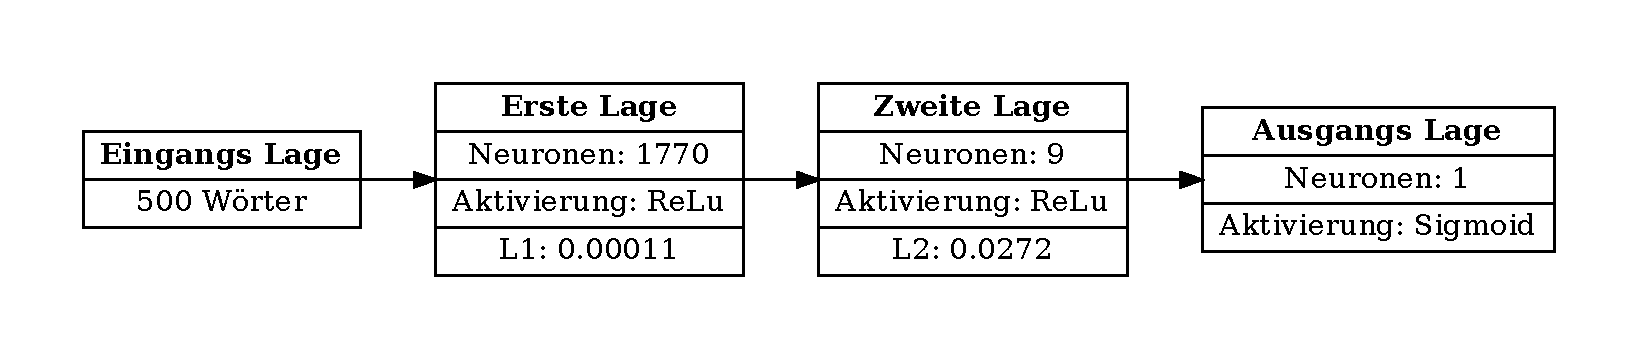
\includegraphics[width=\textwidth]{pictures/modell_scheme.pdf}
    \caption{Grafische Darstellung des optimierten Modells. Es wurden Tiefe, Breite und Regularisierung mithilfe 
            des Tree of Parzen Estimator Algorithmus (siehe \autoref{sec:TPE}) optimiert.}
    \label{fig:NN_structure}
\end{figure}

Das mit Keras\cite{keras} aufgebaute Netz wird mithilfe der \textsc{hyperas}-Bibliothek\cite{hyperas} optimiert und 
es ergibt sich der in \autoref{fig:NN_structure} dargestellte Classifier.
Als Verlustfunktion stellt sich die binäre Kreuzentropie als optimal heraus und als Optimierer der Adagrad Algorithmus.
Bei dem Adagrad Algorithmus werden die Standard Einstellungen verwendet, 
da eine Optimierung der Lern- und Zerfallsrate zu einem unbeständigen Training geführt hat und die Optimierung in einem 
lokalen Minimum endete.


\chapter{Ergebnisse und Interpretation}
\begin{figure}
    \centering
    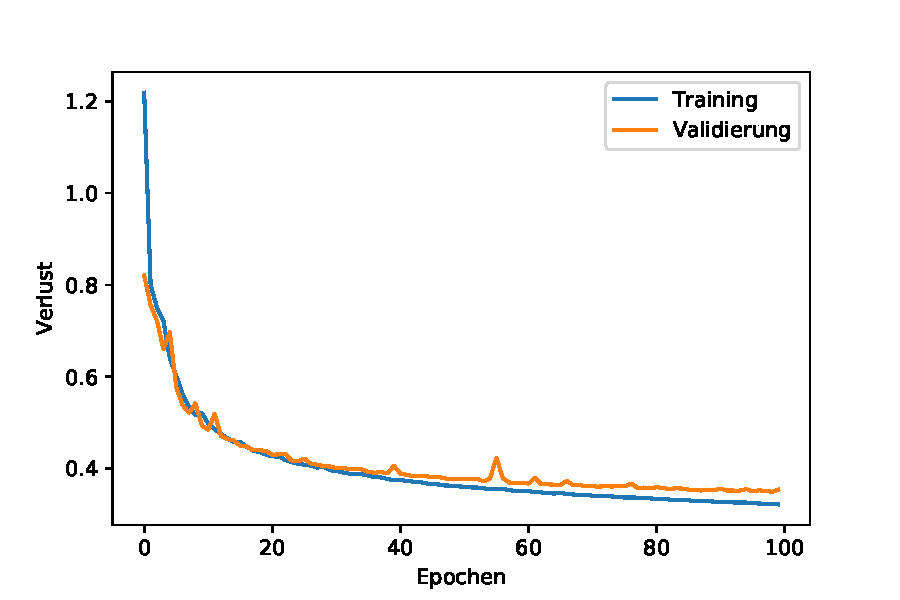
\includegraphics[width=0.7\textwidth]{pictures/history_bow_best.pdf}
    \caption{Abbildung des Trainings- und Validierungsfehlers im Laufe des Trainings. Ein leichtes Übertraining
            ist ab $\approx 40$ Epochen zu erkennen.}
    \label{fig:history}
\end{figure}
\begin{figure}
    \centering
    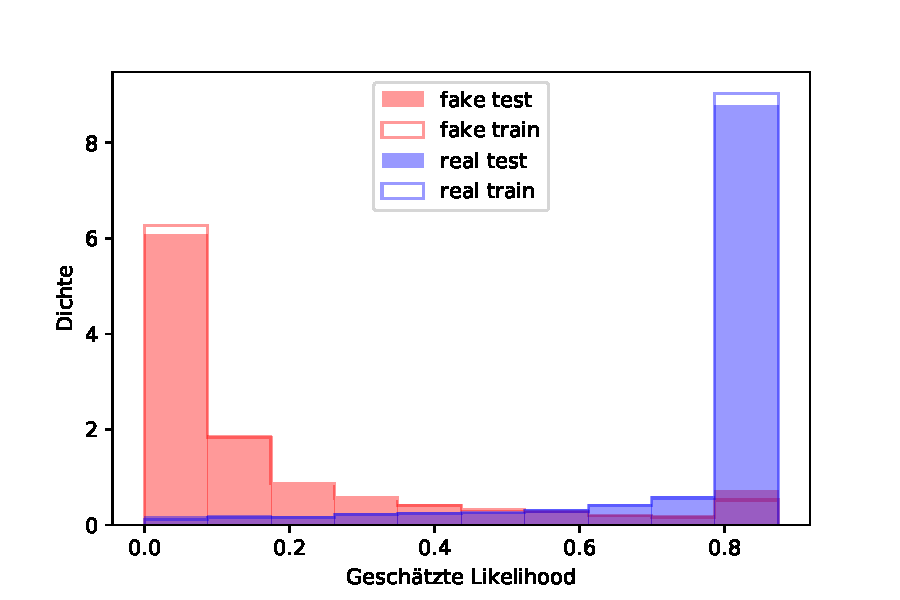
\includegraphics[width=0.7\textwidth]{pictures/prob_bow_best_nn.pdf}
    \caption{Darstellung der Vorhersage bei Trainings und Testdatensatzes. Der Vergleich der Vorhersagen für den 
            Trainings- und Testdatensatz lässt kein Übertraining erkennen. Die Verteilung der Likelihood 
            für die Fake News ist breiter als die der Real News, was zu einer erhöhten Kreuzentropie führt.}
    \label{fig:probs}
\end{figure}

Das Modell wird über $100$ Epochen trainiert und über die Epochen der Trainings- und Validierungsfehler 
berechnet, was in \autoref{fig:history} dargestellt ist. 
Da eine Batch Size von $64$ genutzt wird, ist ein langsames Training zu beobachten, jedoch besitzt die Berechnung 
des Gradienten so weniger Fluktuationen und es ist wahrscheinlicher das globale Minimum zu finden. 
Ab $\approx 40$ Epochen ist das Modell nahezu ausgelernt, da der Validierungsfehler nahezu konstant bleibt und 
nur der Trainingsfehler weiter sinkt.
Für das beste Modell besteht jedoch kein Übertraining, was auch in \autoref{fig:probs} zusehen ist.
Die vorhergesagten Likelihoods sind bei Trainings- und Validierungsdatensatz nahezu gleich verteilt und die 
Genauigkeit für Trainingsdatensatz ist nur leicht über der des Testdatensatzes.
Die Verteilungen sind mit einem Schnitt bei $0.5$ gut zu trennen, was auf eine Genauigkeit von $0.86$ für die 
Fake News Klassifizierung und eine Genauigkeit von $0.90$ für die Real News Klassifizierung führt.
Die Breite der Fake News Verteilung führt jedoch auf eine erhöhte Kreuzentropie von $0.32$.

\begin{figure}
    \centering
    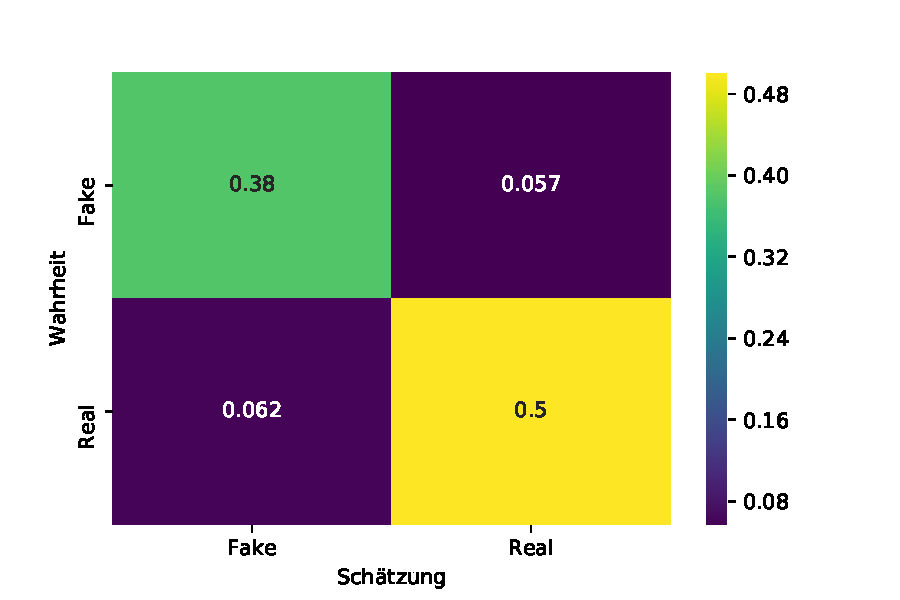
\includegraphics[width=0.7\textwidth]{pictures/cnfsn_mtx_bow_best_nn.pdf}
    \caption{Darstellung der Confusion Matrix, mit klarer Ausprägung der Hauptdiagonalen.}
    \label{fig:CM}
\end{figure}
\begin{figure}
    \centering
    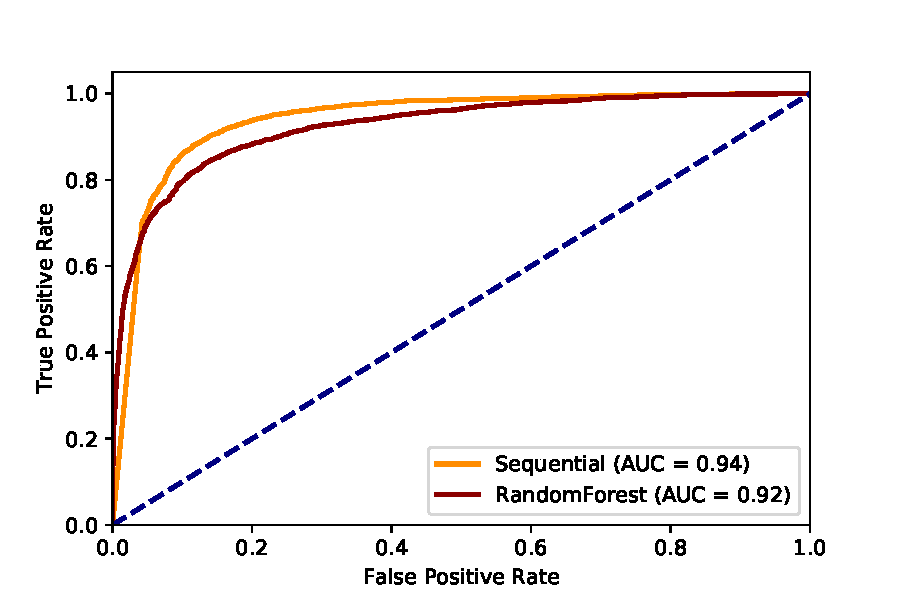
\includegraphics[width=0.7\textwidth]{pictures/roc_comparison.pdf}
    \caption{Die Receiver Operating Characteristic(ROC) für das Neuronale Netzwerk und den Random Forest. Wobei 
            das Neuronale Netz besser klassifiziert, jedoch die Breite der Fake News Verteilung in \ref{fig:probs}
            zu einer schlechteren Performanz des Neuronalen Netzes bei geringen Schwellwerten führt.}
    \label{fig:ROC}
\end{figure}

In \autoref{fig:CM} ist die Vorhersage des Neuronalen Netzes in einer Confusion Matrix dargestellt. 
Da die Nebendiagonalen etwa $12\%$ der Daten beinhalten und beide Diagonalelemente(True Positive und True Negative) 
relativ zum Datenanteil der Wahrheiten gleichermaßen ausgeprägt sind, kann von einem erfolgreichen Training gesprochen 
werden.
Auch die Receiver Operating Characteristic(ROC) in \autoref{fig:ROC} mit einem Area under Curve(AUC) Wert von $0.94$ spricht dafür, dass 
der Classifier eine Struktur in den Daten erkannt hat.
Die ROC Kurve zeigt auch die Schwäche des Modells bei der Erkennung von Fake News, hier an der schlechten 
Performanz für niedrige Schwellwerte zu sehen.
Dies ist auch in \autoref{fig:probs} zusehen und führt auf die erhöhte Kreuzentropie.

\begin{figure}
    \centering
    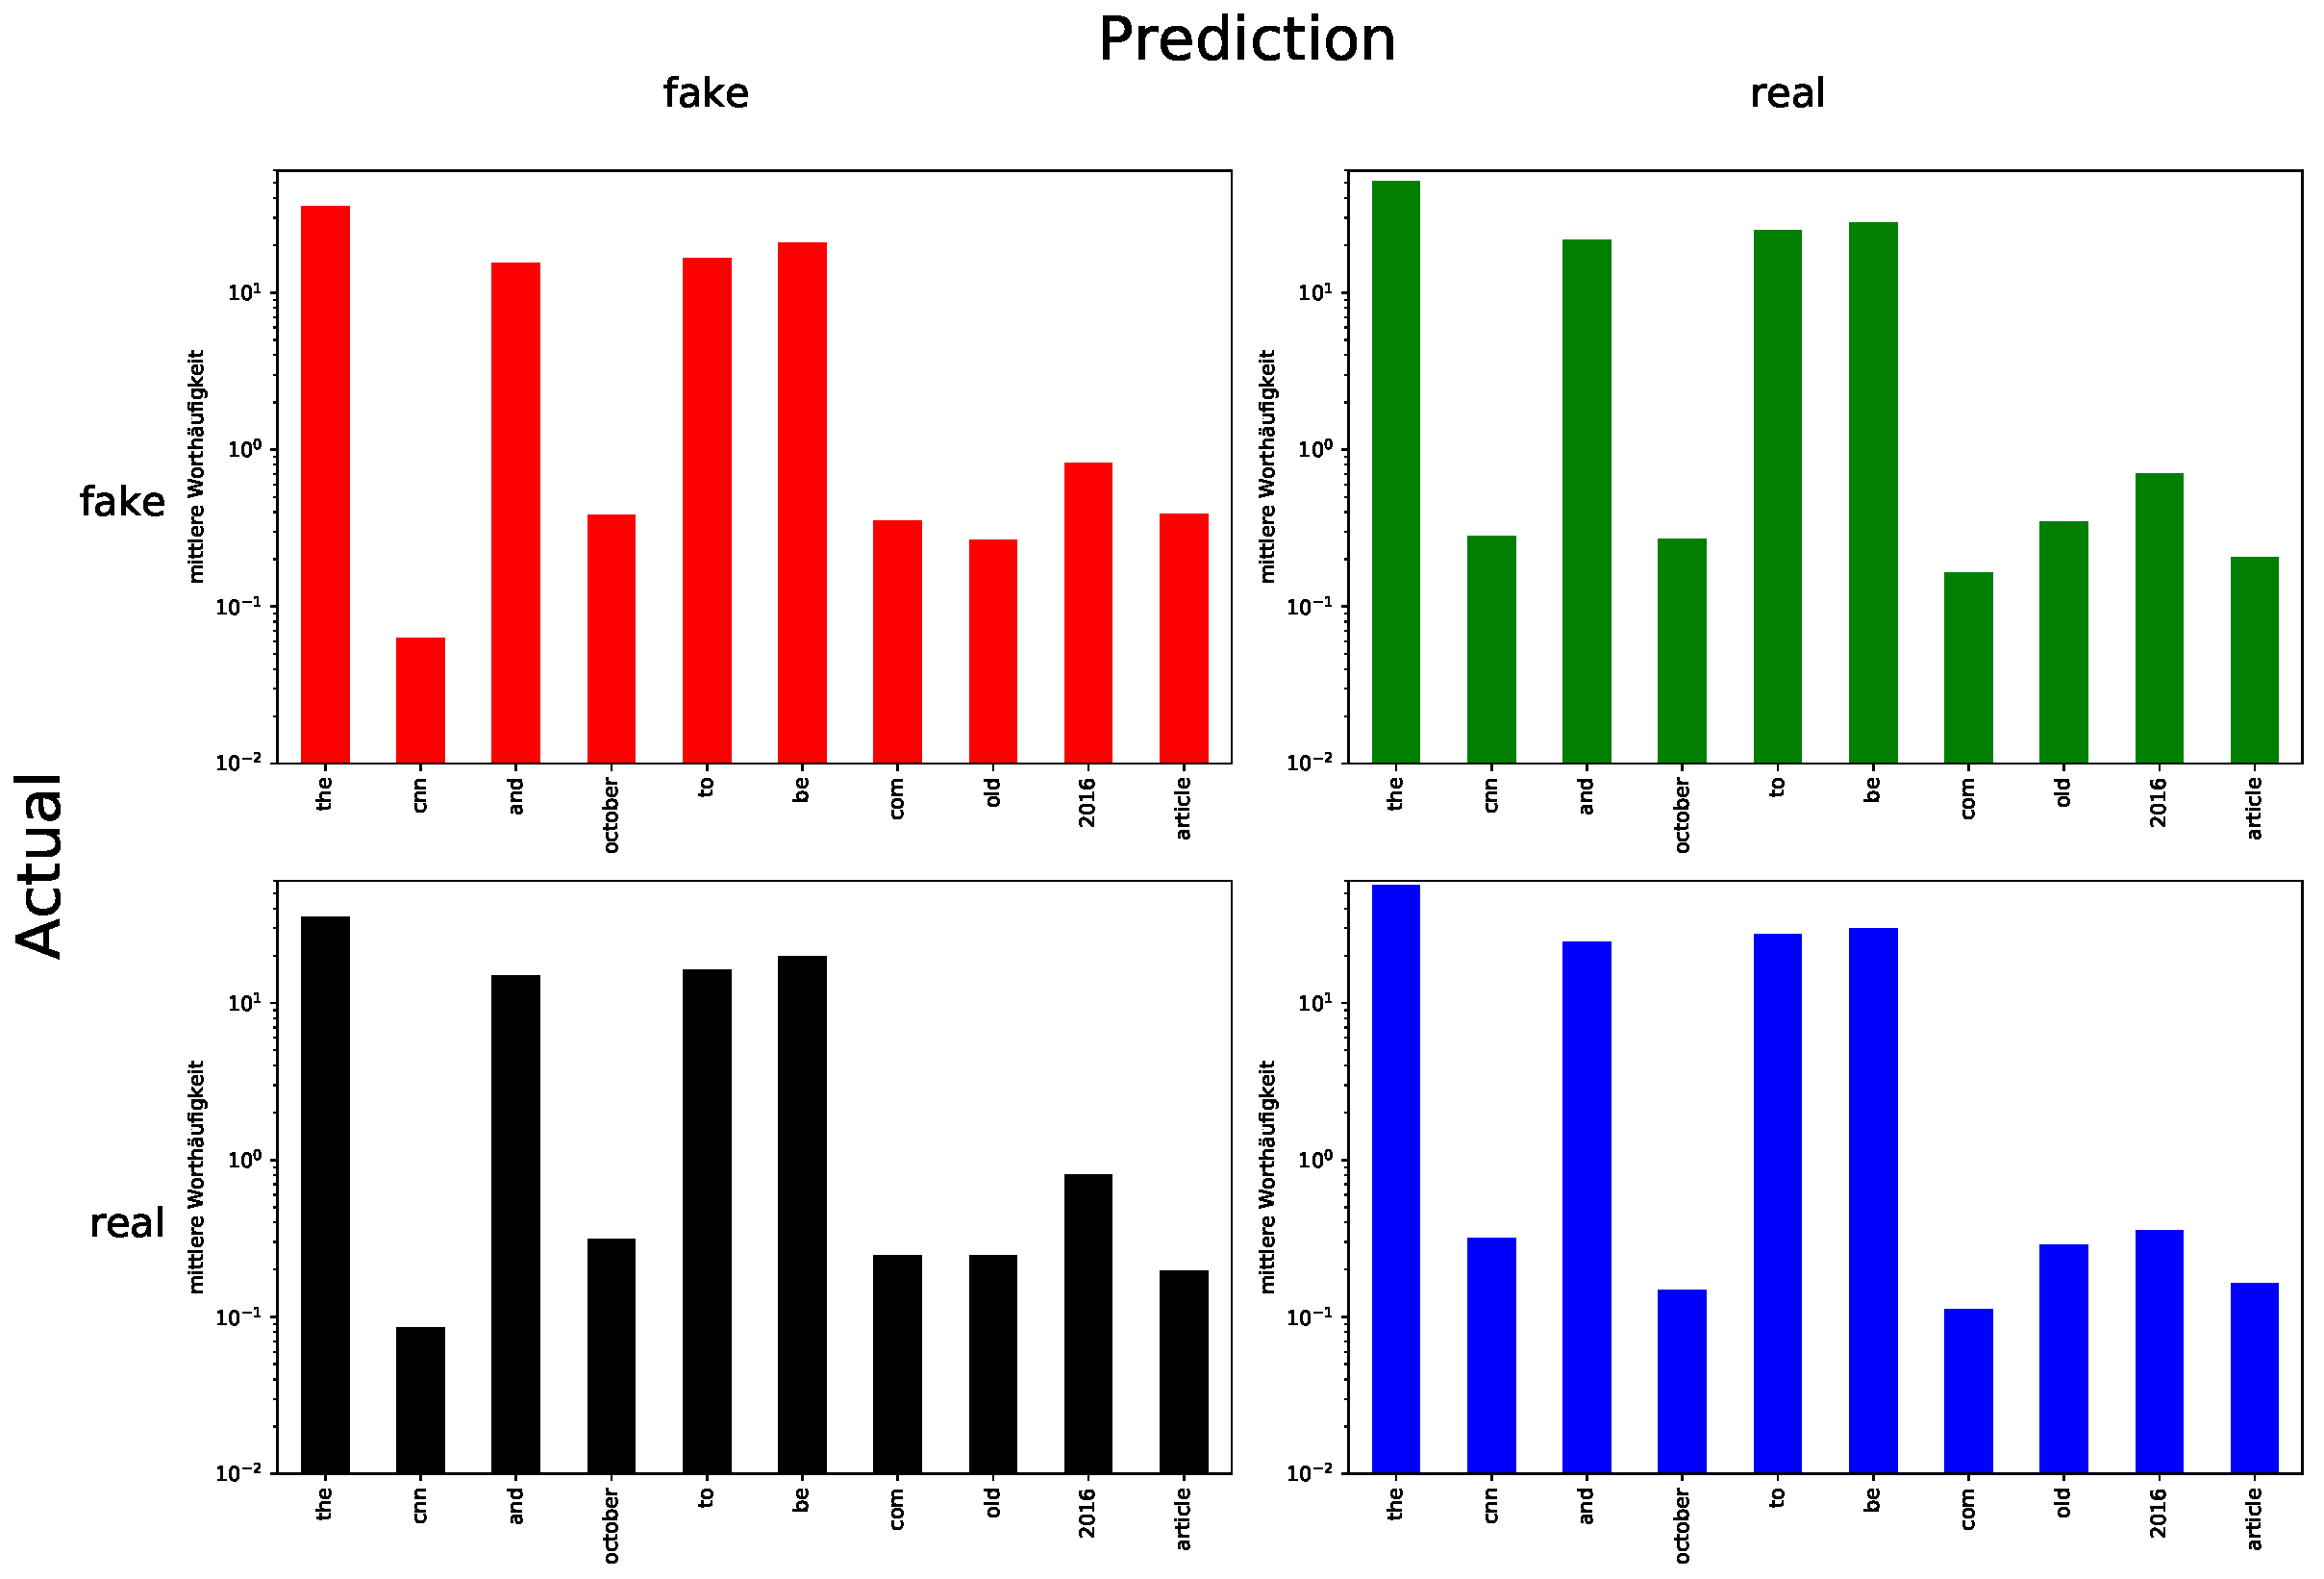
\includegraphics[width=\textwidth]{pictures/cnfn_hist.pdf}
    \caption{Untersuchung der Fehlklassifizierungen mithilfe der Worthäufigkeiten von Worten, denen vom 
            Modell eine hohe Wichtigkeit beigemessen wird.}
    \label{fig:CM_i}
\end{figure}

Um die Trennung besser zu verstehen, wird die erste Lage des Neuronalen Netzes genauer untersucht.
Dabei wird
\begin{equation}
    g_i = \sum_{j=1}^{N_2}|w_{ij}|
\end{equation}
als Wichtigkeit des Wortes $w_i$ interpretiert. Dabei ist $w_{ij}$ das Gewicht von Attribut $i$ zum Neuron $j$ der 
ersten versteckten Lage und $N_j=1770$ die Breite dieser Lage.
Die mittlere Häufigkeit der $10$ wichtigsten Worte werden in \autoref{fig:CM_i} für die richtig und falsch klassifizierten 
Texte dargestellt.
Deutlich zu erkennen ist, dass die Histogramme bei der gleichen Schätzung eine fast gleiche Struktur besitzen, was 
die Fehlklassifizierung erklärt.
Wie schon in \autoref{sec:ansatz} vermutet, spielen Stoppwörter wie "the", "to", "and" und "be" eine zentrale Rolle in der Trennung.
Die Stoppwörter sind klar mit der Textlänge korreliert und da Texte der Real News im Mittel $\num{1590}$ Zeichen 
länger sind, klassifiziert das Modell, wie in \autoref{fig:CM_i} zu sehen, Texte mit einer höheren Worthäufigkeit bei Stoppwörtern 
als Real News.
Das Wort "cnn" wird von dem Neuronalen Netz auch als Indiz für einen Real News Text gesehen.
Dies ist vielleicht damit zu begründen, dass wahre und seriöse Nachrichten sich auf Quellen, wie CNN beziehen und 
Falschmeldungen keine seriöse Quelle besitzen.
Das Wort "com" ist ein Indiz auf Internetseiten und kommt in Texten die als Fake News klassifiziert werden häufiger 
vor.
Zum einen kann das daran liegen, dass Fake News häufiger Internetquellen nutzen, jedoch liegt es auch daran, dass die 
im Datensatz benutzten Fake News Texte einen freiere blogähnliche Schreibstruktur aufweisen. 
Im Gegensatz zu der seriösen und strikten Bericht Struktur der Nachrichten aus den seriösen Nachrichtendiensten.
In \autoref{fig:CM_i} ist auch zu erkennen, dass die $10$ Wörter in einer der beiden Kategorien im Schnitt mindestens in 
jedem fünften Text vorkommen, was auf eine Generalisierung hindeutet.
Das Wort "2016" ist jedoch klar zeitbezogen, wodurch Texte aus einem anderen 
Zeitraum für das trainierte Modell deutlich schwerer zu klassifizieren sind. 

Um Beurteilen zu können, ob das aufwendige Training eines tiefen Neuronalen Netzes notwendig ist oder ob eine einfachere
Methode des Maschinellen Lernens ähnliche Ergebnisse liefert, wird in \autoref{fig:ROC} zusätzlich die Performanz eines 
Random Forests dargestellt.
Der Random Forest nutzt genau wie das Neuronale Netz die Worthäufigkeiten des Bag of Words Modells, jedoch 
werden Schnitte in den Merkmalen verwendet, um die Daten zu klassifizieren.
Für das Training wird der Random Forest aus der \textsc{scikit-learn}-Bibliothek\cite{scikit-learn} verwendet.
Der trainierte Random Forest besitzt $100$ Entscheidungsbäume mit einer maximalen Tiefe von $10$ und als Trennkriterium wird die 
Informationsentropie verwendet.
\autoref{fig:ROC} zeigt, dass das Neuronale Netz mit einem AUC Wert von $0.94$ besser klassifiziert als der Random Forest
mit einem AUC Wert von $0.92$.
Jedoch erkennt der Random Forest die Fake News mit einer Genauigkeit von $0.87$ wie das Neuronale Netz und ist, wie 
in der ROC Kurve zu sehen für sehr niedrige Schnitte besser.
Jedoch ist die Genauigkeit bei der Erkennung der Real News mit $0.81$ schlechter als die Genauigkeit des Neuronalen 
Netzes mit $0.90$. 
Da in die Hyperparameter Optimierung des Random Forests weniger Zeit wie in die Optimierung des Neuronalen 
Netzes investiert wurde, kann nicht zwingend von einer Überlegenheit des Neuronalen Netzes gesprochen werden.


\chapter{Zusammenfassung und Diskussion}
Abschließend ist festzustellen, dass eine Fake News Erkennung anhand von Worthäufigkeiten in den Nachrichten möglich 
ist.
Eine durchschnittliche Genauigkeit von $0.88$ lässt darauf schließen, dass Unterschiede in Fake und Real News erfasst
werden können.
Jedoch zeigt \autoref{fig:probs} und \autoref{fig:CM_i} deutlich, dass einige Falschnachrichten große 
Ähnlichkeiten mit wahren Nachrichten haben und somit schwer zu klassifizieren sind.

Auch die schon in \autoref{sec:struct} erwähnten Einschränkungen in der Definition der Fragestellung dürfen nicht 
vergessen werden.
Die Etikettierung des Datensatzes mithilfe des B.S. Detektors ist keine wahre Fake News Erkennung, da nicht der 
Wahrheitsgehalt der Texte überprüft wird, sondern nur eine schwarze Liste von fragwürdigen URLs zur Klassifizierung 
verwendet wird.
Daher sind die in diesem Datensatz als Fake News klassifizierten Nachrichten nicht zwangsläufig Falschnachrichten. 
Die Klassifizierung, die in dieser Arbeit vorgenommen wird, ist viel mehr ein Filter, der Texte von 
vertrauenswürdigen Zeitungen und Artikel von Webseiten mit Verbindungen zu URLs auf der Schwarzen Liste trennt.

Zudem kann der Schreibstil und die Struktur der Texte aufgrund der unterschiedlichen Herkunft 
durchaus abweichen.
Dass das Neuronale Netz die Textstruktur berücksichtigt, ist durch die Wichtigkeit der Stoppwörter in \autoref{fig:CM_i}
zu erkennen.
Die Frage, ob der Unterschied in Stil und Struktur eine Verzerrung im Datensatz bewirkt oder ob dies ein 
legitimes Merkmal darstellt, ist schwer zu beantworten.
Jedoch sind wahre Nachrichten, die keine Artikel ähnliche Struktur aufweisen, in dem Trainingsdatensatz nicht 
vorhanden und somit kann das Neuronale Netz nur Real News dieser Struktur erkennen.
Das Netz ist zum Beispiel nicht auf Kurznachrichten trainiert und wird daher Probleme bei dieser Form der Nachrichten 
haben.


Eine klare Verzerrung, die in diesem Datensatz besteht, ist die Tatsache, dass die Daten in einem festen 
Zeitraum aufgenommen wurden.
Da jedoch die Thematik der Nachrichten in einem anderen Zeitraum variieren kann, wird das 
Modell Nachrichten mit anderer Thematik schlechter trennen können.
Die Wichtigkeit der Zahl "2016" ist ein Indiz dafür, dass das Neuronale Netz die Thematik durchaus berücksichtigt.
\autoref{fig:CM_i} zeigt jedoch auch, das durchaus von einer Generalisierung gesprochen werden kann und nicht nur 
die Thematik als Kriterium genutzt wird.

Da die Performanz des Random Forests nahe an der des Neuronalen Netzes liegt und der Bau des Entscheidungsbaumes 
nur eine Zeitkomplexität von $\Omega(n \log^2 (n))$\cite[96]{understanding_RF} besitzt, ist die Notwendigkeit des 
Trainings eines tiefen Netzes nicht zwangsläufig gegeben.
Jedoch könnte ein größerer Datensatz und mehr Rechenkapazität das Potenzial des Neuronale Netz mehr ausschöpfen.
Auch andere NLP Methoden wie "word2vec" oder der BERT Encoder\cite{bert} sind vielversprechende Methoden, die jedoch 
größere Neuronale Netze benötigen. 
Eine einfache Analyse der Nachrichten Überschriften mithilfe des BERT Encoders und eines feedforward Neuronalen 
Netzes besitzt schon eine Genauigkeit von $0.77$. 
Die Verarbeitung von ganzen Texten ist jedoch zu rechenaufwendig für dieses Projekt und konnte nicht weiter 
verfolgt werden.
Eine andere vielversprechende Methode sind rückkoppelnden Neuronalen Netze, welche auch auf gute vorläufige Ergebnisse 
geführt haben.
Beide Methoden besitzen die Möglichkeit den Kontext des Textes und nicht allein die Worthäufigkeiten bei der 
Trennung mit zu berücksichtigen, jedoch ist eine Interpretation der Trennung deutlich schwieriger bis nicht möglich.

Aufgrund der genannten Kritikpunkte ist deutlich geworden, dass eine Fake News Detektion anhand der Worthäufigkeiten 
durchaus Probleme birgt und das der genutzte Datensatz auch Schwachstellen besitzt.
Eine mühsame Überprüfung des Wahrheitsgehalts der Texte ist unabdingbar, um eine faire Detektion durchzuführen.
Jedoch sind die Methode des Maschinellen Lernens durchaus in der Lage eine schnelle 
vorläufige Fake News Warnung auszugeben, die, wie in \autoref{sec:motivation} beschrieben, eine unaufhaltsame 
Verbreitung verhindern könnte.


\appendix
\chapter{Natural Language Processing}
\label{sec:NLP}
Bei Methoden des Natural Language Processing geht es darum Texte und Sprache maschinell zu Verarbeiten. Dabei 
sollen nicht nur Wörter, sondern auch in Sätze und ganze Texte die Bedeutung zu erfassen und zu verarbeiten. 
Die Methode des Bag-of-words, die in dieser Arbeit verwendet wird, ist eine Darstellung des Textes anhand der 
Worthäufigkeiten. 
Dabei können das Vokabular und die Häufigkeit von bekannten Wörtern extrahiert werden. 
Mit dieser Methode kann jedoch nicht die Bedeutung der Worte extrahiert werden und außerdem werden viele Wörter 
extrahiert, die keine Information für die Lösung des eigentlichen Problems beinhalten müssen. 
Dies führt auf einen zu großen Suchraum, der durch Beschränkung der Wörterauswahl manuell verkleinert werden kann.

Um Wörter unterschiedlicher Flexion auf ihre Grundform zurückzuführen wird das Lemmatisieren verwendet. 
Dabei werden Datenbanken verwendet, um für die Flexionsform die passende Stammform zu finden.

Weiter Methoden, um auch die Bedeutung von Wörtern und Sätzen zu erfassen, sind die "word2vec" Methode und Bidirektionale Satz-Encoder, 
wie das vortrainierte BERT Modell von Google\cite{bert}. Beide Methoden sind Encoder, die Wörter oder Sätze ihrer 
Bedeutung entsprechend in einem hochdimensionalen Hyperraum abbilden. Damit können Beziehungen und Bedeutungen 
von Texten erfasst werden.


\chapter{Bayesian Optimization}
\label{sec:TPE}
Bayesian Optimization ist eine Methode zur Optimierung von Funktionen, die nur anhand ihrer Eingangs $x$ und Ausgangs $y$
Werten definiert sein müssen (Black-Box Funktionen). 
Der Algorithmus schätzt die posterior Verteilung $p(y|x)$ der unbekannten Funktion mithilfe eines Priors $p(y)$, welcher 
nach jeder Funktionsevaluierung neu geschätzt wird.
Der Tree of Parzan Estimator modelliert die Likelihood $p(x|y)$ der Observable $x$ mithilfe des nicht parametrischen 
Dichteschätzers 
\begin{equation}
p(x | y)=\left\{\begin{array}{ll}{\ell(x)} & {\text { if } y<y^{*}} \\ {g(x)} & {\text { if } y \geq y^{*}}\end{array}\right. \text{\, .}
\end{equation}
$\ell(x)$ ist die Dichte von allen zur Zeit evaluierten Beobachtungen $x_i$ mit $f(x_i)<y^{*}$ und 
$g(x)$ ist die Dichte für $f(x_i) \geq y^{*}$. 
Dabei wird $y^{*}$ so gewählt, dass $p\left(y<y^{*}\right)=\gamma$ für ein Quantil $\gamma$ gilt.
Mithilfe des Satzes von Bayes kann anschließend die posterior Verteilung geschätzt werden.

Die Methoden der Baysian Optimization haben den Vorteil, dass sie weder die Ableitung der Zielfunktion noch die
Zielfunktion selbst kennen müssen. 
Jedoch nutzen sie vorhandenes Prior Wissen für die Optimierung und sind somit effizienter wie eine Brute-Force Methode.

\chapter{code}
Der Code für das Modell dieses Berichts ist in dem beigefügten .zip File zu finden. 

Das ganze Projekt mit zusätzlichen Modellen, befindet sich auf github unter https://github.com/Cl3V0r/MLSeminar,
jedoch sind nicht zwangsläufig alle Skripts in diesem Repository optimiert.


% Hier beginnt der Anhang, nummeriert in lateinischen Buchstaben
%\input{a_anhang.tex}

\backmatter
\printbibliography

\end{document}
